\documentclass[class=report,crop=false, 12pt]{standalone}
\usepackage[screen,nosolutions]{../myscratch}
%\usepackage[screen]{../myscratch}



\begin{document}

\titre[S]{Coordonnées $x,y$}
%===============================

\insertvideo{bZGv9CRfkuI}{Coordonnées $x,y$ -- Activité 1}

\insertvideo{3_MUTUTAHJg}{Coordonnées $x,y$ -- Activité 2}

\insertvideo{-FGNNU4qdMw}{Coordonnées $x,y$ -- Activité 3}

\bigskip
\bigskip


\begin{activite}

Essaie de reproduire la spirale suivante.

\begin{center}
  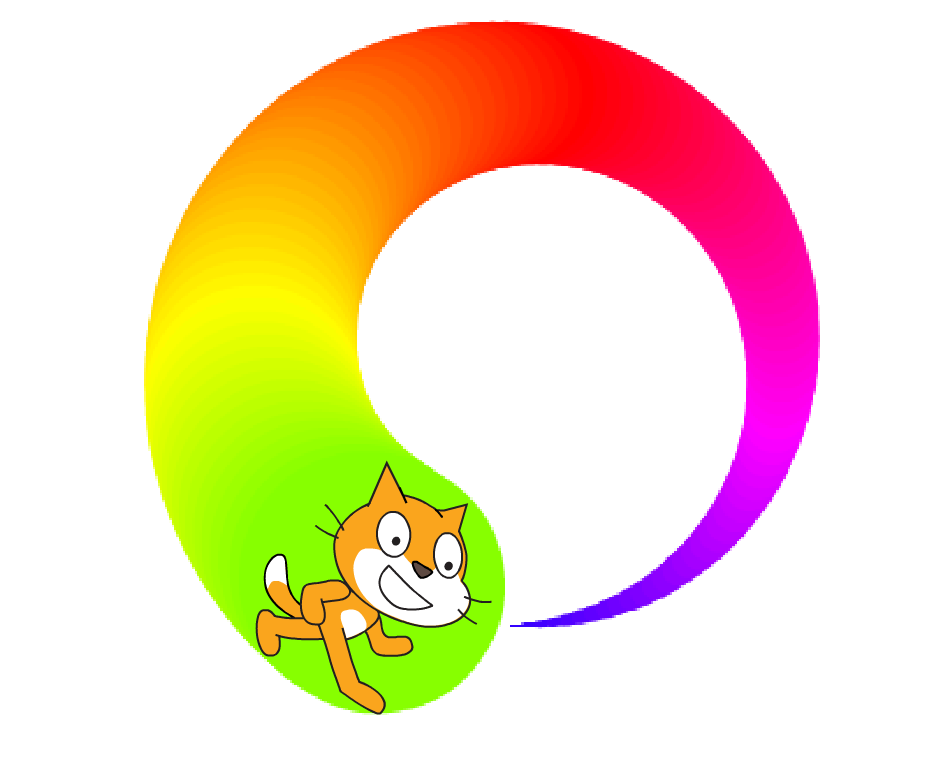
\includegraphics[width=0.6\textwidth]{ecran-03-ex1}   
\end{center}

Au départ la taille du stylo est 1.
Fais une boucle dans laquelle à chaque étape :
\begin{itemize}
  \item tu fais avancer Scratch de 6 pas,
  \item tu fais tourner Scratch de 3 degrés vers la gauche,
  \item tu ajoutes 1 à la taille du stylo,
  \item tu ajoutes 1 à la couleur du stylo.
\end{itemize}


Trouve une bonne position $x,y$ de départ afin que la spirale tienne entièrement dans l'écran.



%\textbf{Blocs utiles.}
%\begin{itemize}
%  \item 
%  
%  \item 
%  
%  
%\end{itemize}

\end{activite}


\begin{activite}
Tu vas programmer ton premier logiciel de dessin.

\begin{center}
  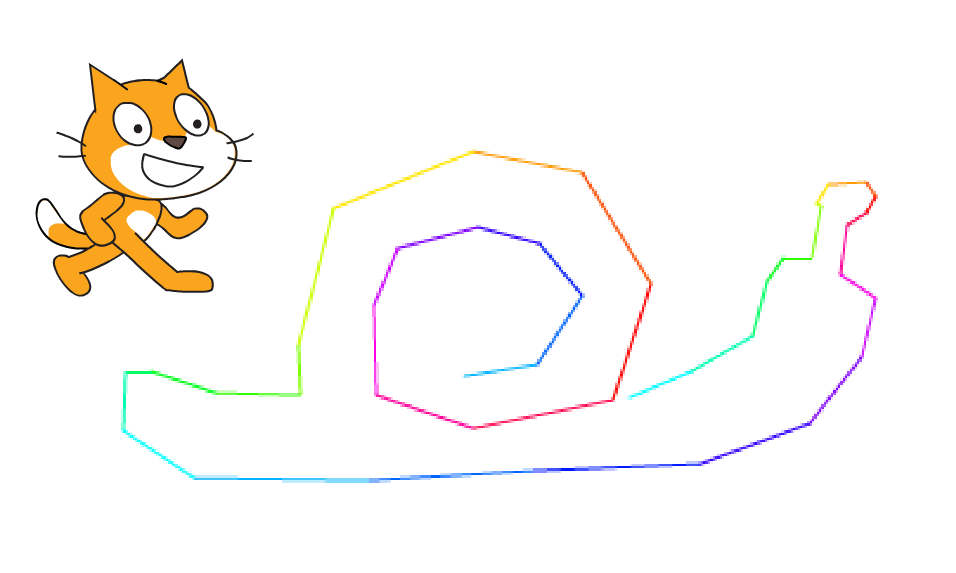
\includegraphics[width=0.55\textwidth]{ecran-03-ex2}   
\end{center}

Pour cela, construis une boucle qui répète indéfiniment :
\begin{itemize}
  \item aller au pointeur de la souris,
  \item afficher l'abscisse $x$ pendant 1 seconde,
  \item afficher l'ordonnée $y$ pendant 1 seconde.
\end{itemize}

Essaie de dessiner un escargot, une maison, une fusée...

\bigskip

\textbf{Blocs utiles.}
\begin{itemize}
  \item \og{}aller à pointeur de la souris\fg{}
  \item \og{}dire abscisse $x$ pendant 1 seconde\fg{}
\end{itemize}

{
\setscratch{scale=0.8}
On obtient le bloc 
\begin{scratch}
\blocklook{dire \ovalmove{ abscisse x} pendant \ovalnum{1} secondes}
\end{scratch}
en insérant le bloc \ovalmove{ abscisse x} à la place de \og{}Bonjour!\fg{} par un \og{}cliqué-déposé\fg{} dans le bloc : 
\begin{scratch}
\blocklook{dire \ovalnum{ Bonjour!} pendant \ovalnum{1} secondes}
\end{scratch}
}

\bigskip

\textbf{Bonus.}
\begin{itemize}
  \item Change de couleur à chaque segment.
  \item Affiche $x$ et $y$ en même temps.
\end{itemize}

    \textbf{Blocs utiles.} Voici deux façons de faire dire à Scratch deux mots. Soit l'un après l'autre, soit en regroupant les deux mots en une seule phrase.
\begin{center}
\begin{scratch}
  \blocklook{dire \ovalnum{ Coucou} pendant \ovalnum{1} secondes}
  \blocklook{dire \ovalnum{ le monde} pendant \ovalnum{1} secondes}
  \blockspace
  \blocklook{dire  
     \ovaloperator{regrouper \ovalnum{ Coucou} et \ovalnum{ le monde}}
     pendant \ovalnum{2} secondes}
\end{scratch}
\end{center}

\end{activite}


\begin{activite}

Choisis comme arrière-plan la grille de coordonnées.

\begin{enumerate}
  \item Trace le chiffre \og \mot{4} \fg{} en suivant les instructions suivantes :
  \begin{itemize}
    \item relever le stylo,
    \item aller à $x=40$, $y=120$,
    \item stylo en position d'écriture,
    \item aller à $x=0$, $y=40$,
    \item aller à $x=80$, $y=40$,
    \item relever le stylo,
    \item aller à $x=60$, $y=20$,
    \item stylo en position d'écriture,
    \item aller à $x=60$, $y=60$.  
  \end{itemize}
  
\begin{center}
  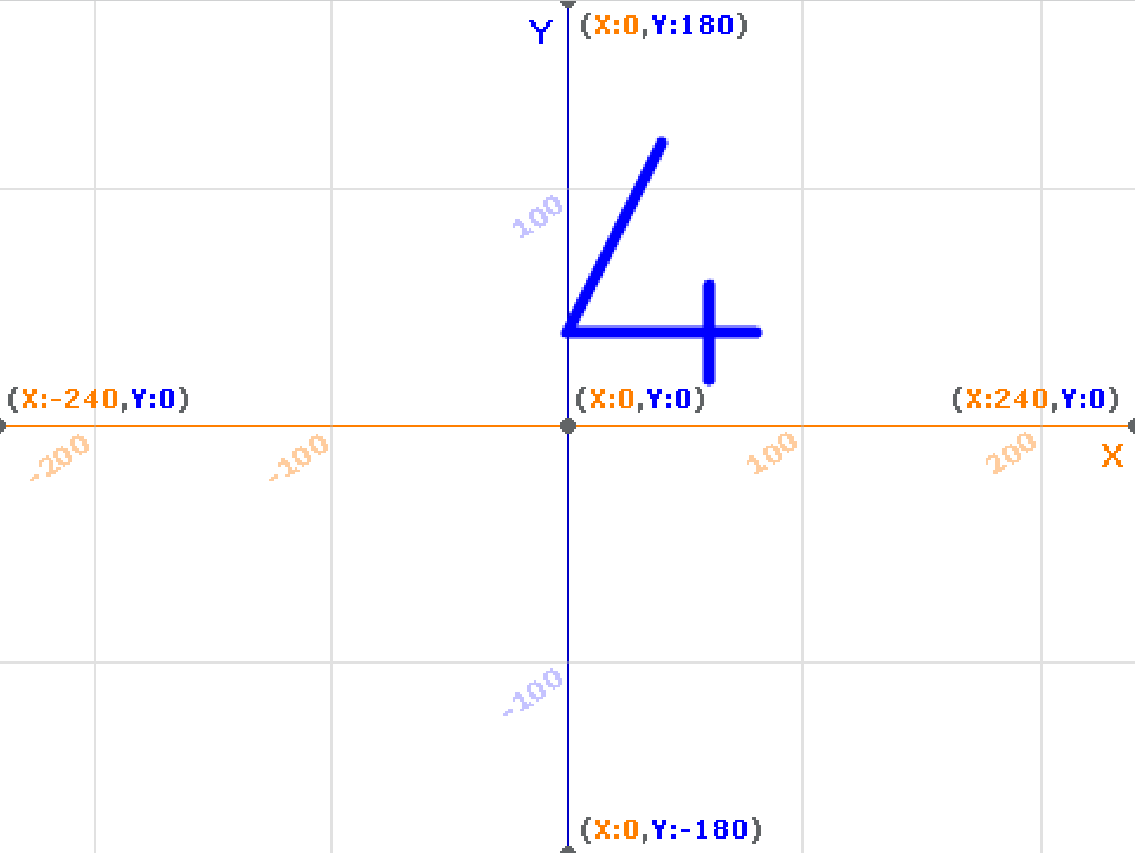
\includegraphics[width=0.55\textwidth]{ecran-03-ex3}   
\end{center}
  
  \item Trace le chiffre \og \mot{7} \fg{} en t'aidant des coordonnées $(x,y)$ des sommets proposés dans le dessin suivant : 
  
\myfigure{0.5}{
\footnotesize\tikzinput{coord1}
}  

  \item Dessine la première lettre de ton prénom en majuscule sur la grille ci-dessous.

\myfigure{1.2}{
\small\tikzinput{coord2}
}  
  
  \item Programme Scratch afin qu'il dessine ton initiale.
  
  
\end{enumerate}


\end{activite}
\vfill\eject

\ifx \displaysolutions \myzero
\else
\begin{code}
  \setscratch{scale=\scalesolution}
  \onesolution{Coordonnées $x,y$}{Activité 1}{
    \begin{scratch}
      \blockinit{quand \greenflag est cliqué}
      \blockmove{aller à x: \ovalnum{50} y: \ovalnum{-100}}
      \blockmove{s'orienter à \ovalnum{90}}
      \blockpen{mettre la taille du stylo à \ovalnum{1}}
      \blockpen{mettre la couleur du stylo à \pencolor{blue!75!black}}
      \blockpen{effacer tout}
      \blockpen{stylo en position d'écriture}
      
      \blockrepeat{répéter \ovalnum{110} fois}
                  {
                    \blockmove{avancer de \ovalnum{6} pas} 
                    \blockmove{tourner \turnleft{} de \ovalnum{3} degrés}
                    \blockpen{ajouter \ovalnum{1} à la taille du stylo}
                    \blockpen{ajouter \ovalnum{1} à la \selectmenu{ couleur} du stylo}
                  } 
    \end{scratch}
  }
  \onesolution{Coordonnées $x,y$}{Activité 2}{
    \begin{scratch}
      \blockinit{quand \greenflag est cliqué}
      \blockmove{aller à x: \ovalnum{0} y: \ovalnum{0}}
      \blockmove{s'orienter à \ovalnum{90}}
      \blockpen{effacer tout}
      \blockcontrol{attendre \ovalnum{1} secondes} 
      \blockpen{stylo en position d'écriture}
      \blockinfloop{répéter indéfiniment}
                   {
                     \blockmove{aller à \selectmenu{pointeur de souris}}
                     \blocklook{dire \ovalmove{ abscisse x} pendant \ovalnum{1} secondes}
                     \blocklook{penser à \ovalmove{ ordonnée y} pendant \ovalnum{1} secondes}
                   }
    \end{scratch}
}
  \onesolution{Coordonnées $x,y$}{Activité 3}{
    \begin{minipage}{0.2\textwidth}
      \hbox{Chiffre 4}
      \begin{scratch}
        \blockinit{quand \greenflag est cliqué}
        \blockpen{effacer tout}
        \blocklook{cacher}
        \blockpen{mettre la taille du stylo à \ovalnum{5}}
        \blockpen{relever le stylo}
        
        \blockmove{aller à x: \ovalnum{40} y: \ovalnum{120}} % \emph{début du chiffre 4}
        \blockpen{stylo en position d'écriture}
        \blockmove{aller à x: \ovalnum{0} y: \ovalnum{40}}
        \blockmove{aller à x: \ovalnum{80} y: \ovalnum{40}}
        \blockpen{relever le stylo}
        \blockmove{aller à x: \ovalnum{60} y: \ovalnum{20}}
        \blockpen{stylo en position d'écriture}
        \blockmove{aller à x: \ovalnum{60} y: \ovalnum{60}}
      \end{scratch}
    \end{minipage}
  }
  \onesolution{Coordonnées $x,y$}{Activité 3}{
    \begin{minipage}{0.2\textwidth}
      \hbox{Chiffre 7}
      \begin{scratch}
        \blockinit{quand \greenflag est cliqué}
        \blockpen{effacer tout}
        \blocklook{cacher}
        \blockpen{mettre la taille du stylo à \ovalnum{5}}
        \blockpen{relever le stylo}
        \blockmove{aller à x: \ovalnum{120} y: \ovalnum{120}} % \emph{début du chiffre 7}
        \blockpen{stylo en position d'écriture}
        \blockmove{aller à x: \ovalnum{200} y: \ovalnum{120}}
        \blockmove{aller à x: \ovalnum{120} y: \ovalnum{20}}
        \blockpen{relever le stylo}
        \blockmove{aller à x: \ovalnum{140} y: \ovalnum{70}}
        \blockpen{stylo en position d'écriture}
        \blockmove{aller à x: \ovalnum{180} y: \ovalnum{70}}
      \end{scratch}
    \end{minipage}
  }    

%  \onesolution{Coordonnées $x,y$}{Activité 2}{
%    \begin{minipage}{0.4\textwidth}
%      \hbox{Bonus}
%      \begin{scratch}
%        \blockinit{quand \greenflag est cliqué}
%        \blockmove{aller à x: \ovalnum{0} y: \ovalnum{0}}
%        \blockmove{s'orienter à \ovalnum{90}}
%        \blockpen{effacer tout}
%        \blockcontrol{attendre \ovalnum{1} secondes} 
%        \blockpen{stylo en position d'écriture}
%        \blockinfloop{répéter indéfiniment}
%                     {
%                       \blockmove{aller à \selectmenu{pointeur de souris}}
%                       \blockpen{ajouter \ovalnum{10} à la \selectmenu{ couleur} du stylo}
%                       \blocklook{dire  
%                         \ovaloperator{regrouper \ovalnum{ abscisse x} et \ovalnum{ ordonnée y}}
%                         pendant \ovalnum{2} secondes}
%                     }
%      \end{scratch}
%    \end{minipage}
%  }
\end{code}
\fi

\end{document}

